\subsection{Building level}

The main components of a typical data center are:
\begin{itemize}
	\item Cooling system (blue):
	\begin{itemize}
		\item Water storage
		\item Cooling towers
		\item Chillers
		\item Fan coil air handling units
	\end{itemize}
	
	\item Power supply (red):
	\begin{itemize}
		\item Utility power
		\item Transformers
		\item Backup generation/power distribution
		\item Power bus
	\end{itemize}
	
	\item Computation storage networking (green):
	\begin{itemize}
		\item Networking room
	\end{itemize}
\end{itemize}

\begin{figure}[!htp]
	\centering
	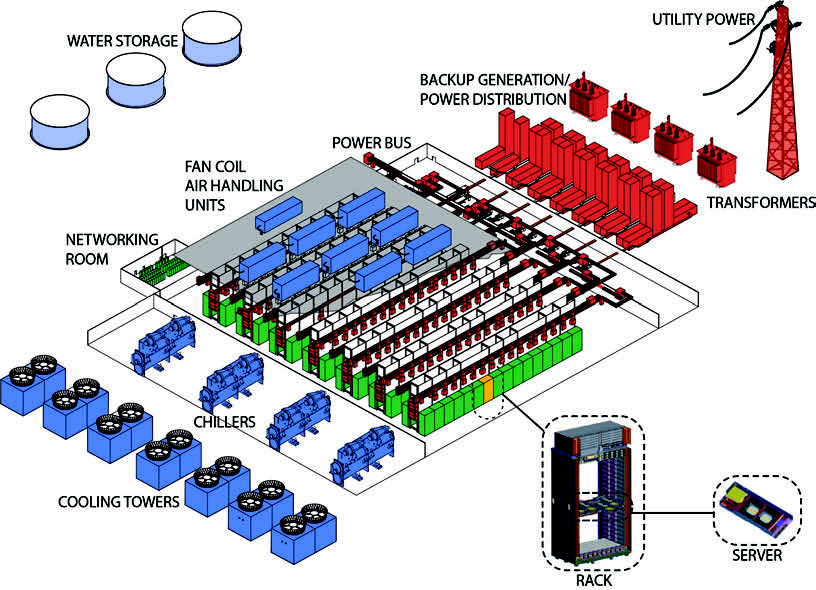
\includegraphics[width=\textwidth]{img/components-dc-1.png}
	\caption{The main components of a typical data center.\cite{barroso2022datacenter}}
\end{figure}

\noindent
The warehouse scale computer or data centre has other important components related to \textbf{power delivery}, \textbf{cooling} and \textbf{building infrastructure} that also need to be considered.

\highspace
In order to protect against power failure, battery and diesel generators are used to back up the external supply.

\highspace
A \definition{UPS (uninterruptible power supply or source)} is a \textbf{continual power system that provides automated backup electric power to a load when the input power source or mains power fails}. There are many types of UPS, but in general, in the DC, the \definition{Rotary UPS system} is used.

\highspace
A rotary UPS uses the inertia of a high-mass spinning flywheel to provide short-term ride-through in the event of power loss.

\begin{figure}
	\centering
	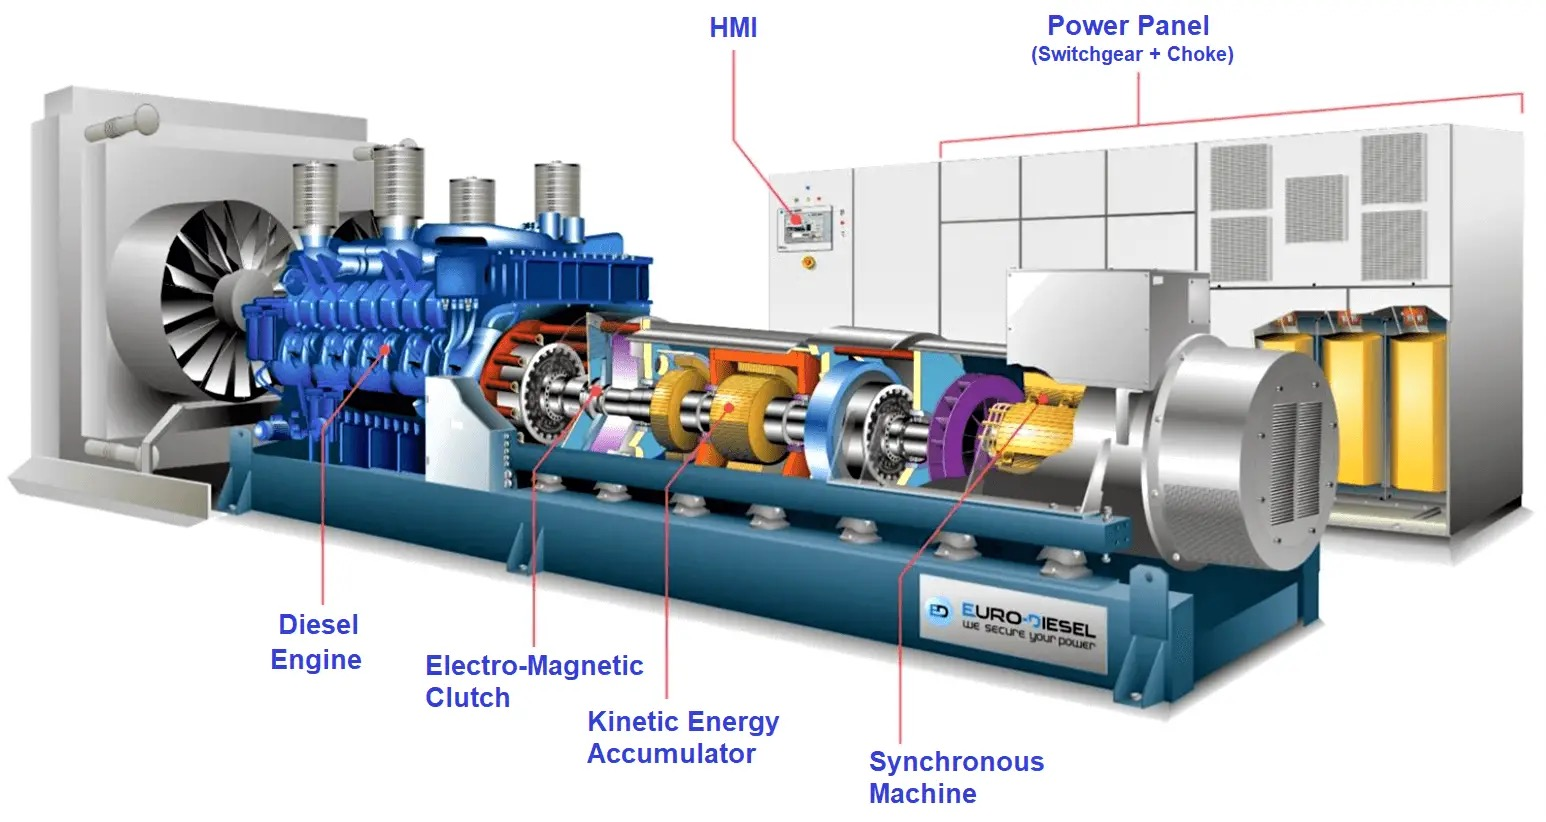
\includegraphics[width=\linewidth]{img/components-dc-2.png}
	\caption{A Rotary UPS system.}
\end{figure}

\newpage

\subsubsection{Cooling systems}

The IT equipment generates a lot of heat. To avoid troubles, cooling systems have been installed. Unfortunately, they are costly components of the data center, and they are composed of \textbf{coolers}, \textbf{heat exchangers} and \textbf{cold water tanks}.

\highspace
Some techniques exist to improve cooling systems without throwing away too much money.

\highspace
\definition{Open-Loop systems} refer to the \textbf{use of cold outside air to either help the production of chilled water or directly cool servers}. It is not entirely free in the sense of zero cost, but it involves \textbf{very low energy costs} compared to chillers.

\highspace
\definition{Closed-Loop systems} come in many forms, the most common being the air circuit on the data centre floor. 
It is grouped by number of loops:
\begin{itemize}
	\item \textbf{\emph{One loop}}. The \textbf{main goal is to isolate and remove heat from the servers and transport it to a heat exchanger}. So the cold air flows to the servers, heats up, and eventually reaches a heat exchanger to cool it down again for the next cycle through the servers.
	\begin{flushleft}
		\textcolor{Green3}{\faIcon{check} \textbf{Advantages}}
	\end{flushleft}
	It can be very efficient.
	\begin{flushleft}
		\textcolor{Red2}{\faIcon{exclamation-triangle} \textbf{Cons}}
	\end{flushleft}
	\begin{itemize}
		\item It doesn't work in all climates;
		\item It requires filtering of airborne particulates;
		\item Can introduce complex control problems.
	\end{itemize}
	
	\item \textbf{\emph{Two loops}}. The airflow through the underfloor plenum, the racks, and back to the \definition{CRAC (computer room air conditioning)} defines the primary air circuit as the first loop. The second loop (the liquid supply inside the CRAC units) leads directly from the CRAC to the external heat exchangers (typically placed on the building roof) that discharge the heat to the environment.
	\begin{flushleft}
		\textcolor{Green3}{\faIcon{check} \textbf{Advantages}}
	\end{flushleft}
	\begin{itemize}
		\item Easy to implement;
		\item Relatively inexpensive to construct;
		\item Offers isolation from external contamination.
	\end{itemize}
	\begin{flushleft}
		\textcolor{Red2}{\faIcon{exclamation-triangle} \textbf{Cons}}
	\end{flushleft}
	Typically have lower operational efficiency.
	\begin{figure}[!htp]
		\centering
		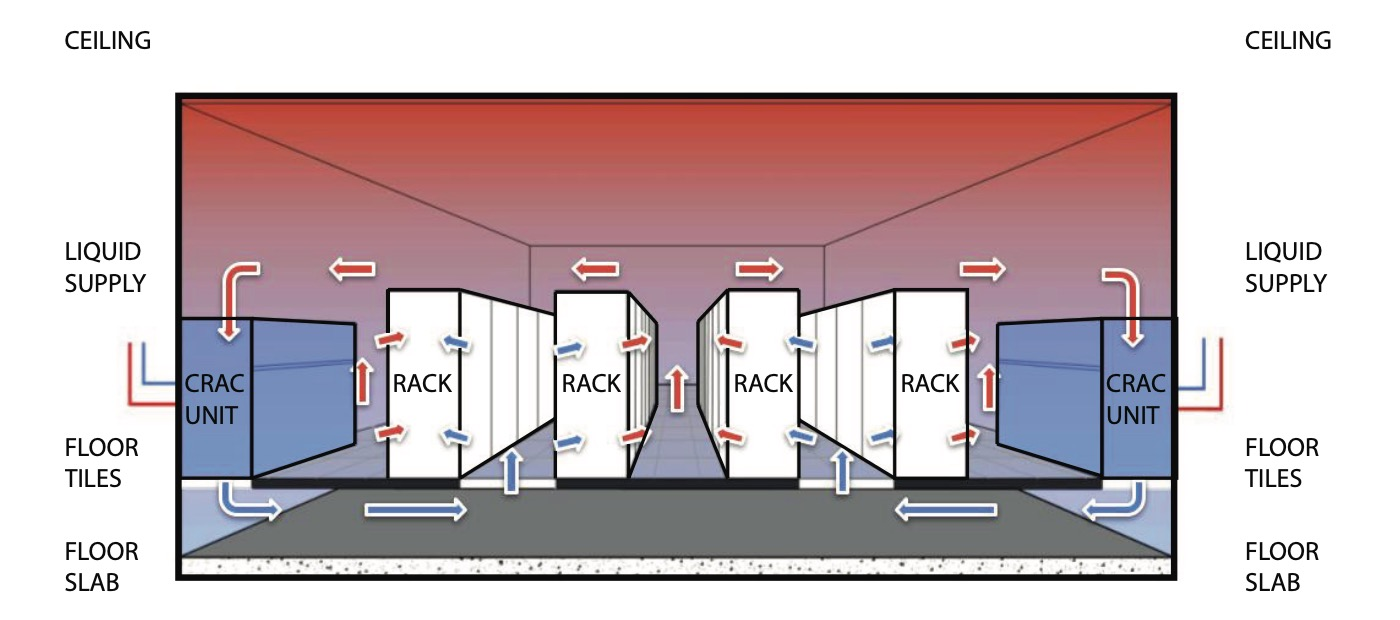
\includegraphics[width=\textwidth]{img/components-dc-3.png}
	\end{figure}
	\newpage
	
	\item \textbf{\emph{Three loops}}. It is used in large-scale data centres. The architecture can be viewed in the following figure.
	\begin{flushleft}
		\textcolor{Green3}{\faIcon{check} \textbf{Advantages}}
	\end{flushleft}
	\begin{itemize}
		\item It offers contaminant protection;
		\item It offers good efficiency.
	\end{itemize}
	\begin{flushleft}
		\textcolor{Red2}{\faIcon{exclamation-triangle} \textbf{Cons}}
	\end{flushleft}
	\begin{itemize}
		\item It is the most expensive to construct;
		\item It has moderately complex controls.
	\end{itemize}
	\begin{figure}[!htp]
		\centering
		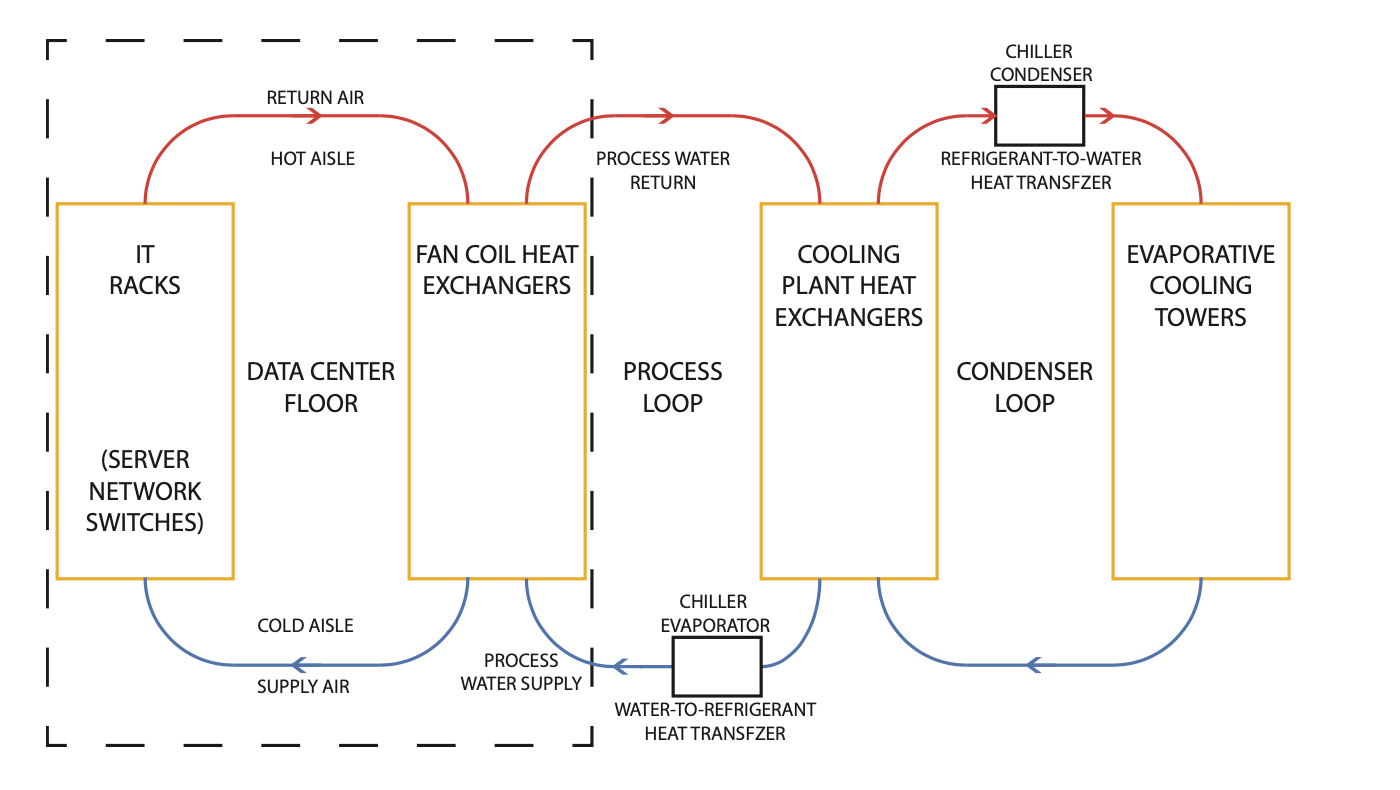
\includegraphics[width=\textwidth]{img/components-dc-4.png}
		\caption*{First loop to the left, second loop in the middle and third loop to the right.}
	\end{figure}
\end{itemize}

\newpage

\begin{flushleft}
	\textcolor{Green3}{\faIcon{question-circle} \textbf{How each rack is cooled?}}
\end{flushleft}
There are three ways to cool each rack:
\begin{itemize}
	\item \definition{In-Rack cooler}. It \textbf{adds an air-to-water heat exchanger} at the \textbf{back of a rack} so the \textbf{hot air exiting the servers immediately flows over coils cooled by water}, reducing the path between server exhaust and CRAC input.
	
	\item \definition{In-Row cooling}. It works like in-rack cooling, except the \textbf{cooling coils} are not in the rack but \textbf{adjacent to the rack}.
	\begin{figure}[!htp]
		\centering
		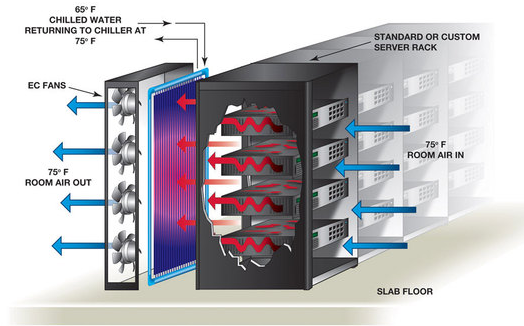
\includegraphics[width=\textwidth]{img/in-row-cooling-1.png}
		\caption{In-Row Cooling Mechanism (source: \href{https://www.energystar.gov/products/data_center_equipment/16-more-ways-cut-energy-waste-data-center/install-rack-or-row}{Energy Start}).}
	\end{figure}
	
	
	\item \definition{Liquid cooling}. We can directly \textbf{cool server components using cold plates}. The \textbf{liquid circulating through the heat skins transports the heat to a liquid-to-air or liquid-to-liquid heat exchanger} that can be placed close to the tray or rack or be part of the data centre building (such as a cooling tower).
	\begin{figure}[!htp]
		\centering
		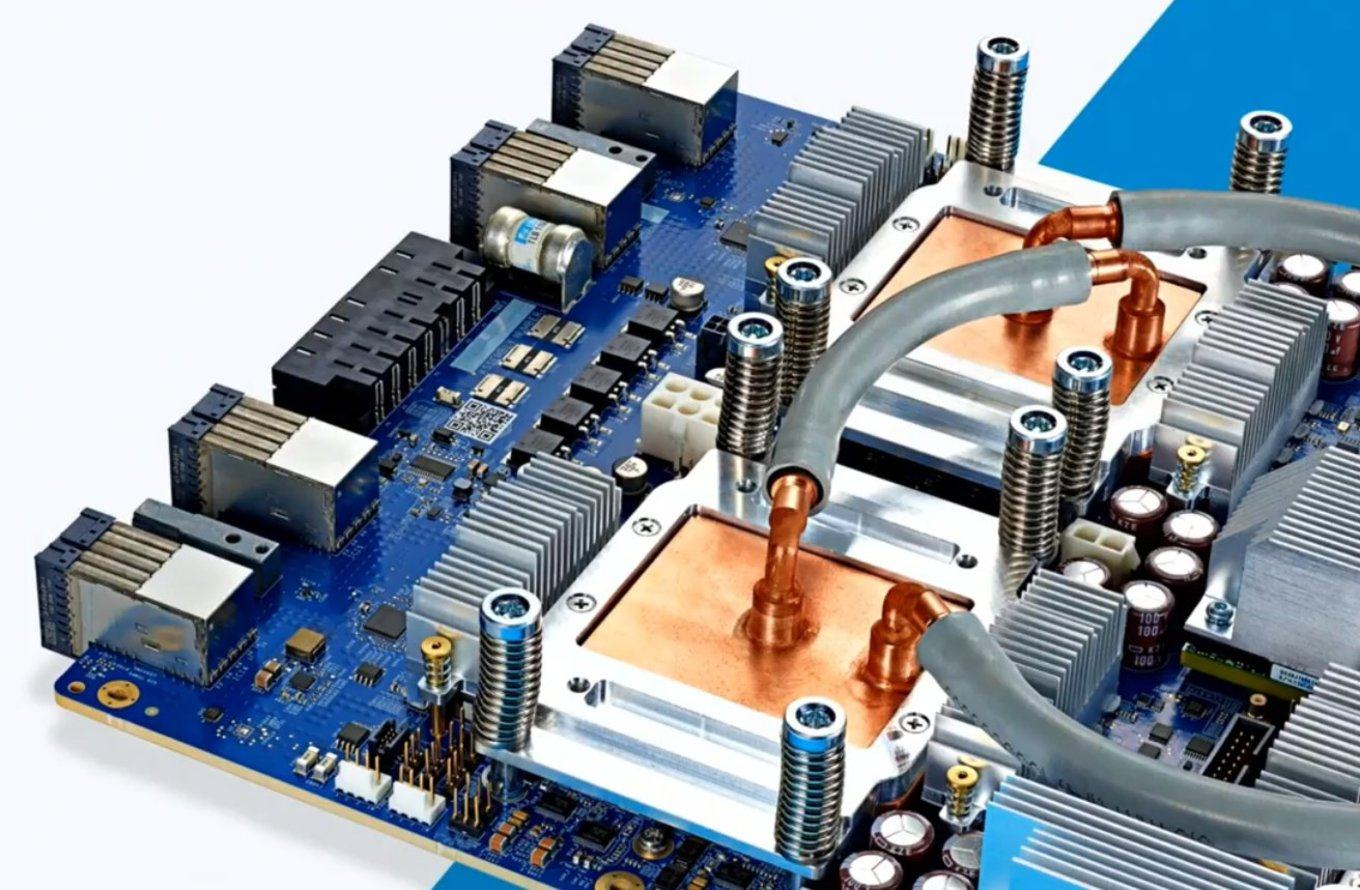
\includegraphics[width=.45\textwidth]{img/liquid-cooling-1.jpg}
		\caption{Liquid Cooling Mechanism.}
	\end{figure}
\end{itemize}

\newpage

\subsubsection{Power supply}

\begin{flushleft}
	\textcolor{Green3}{\faIcon{question-circle} \textbf{What is the problem?}}
\end{flushleft}
Data centre power consumption is an issue since it can reach several milliwatts. \textbf{Cooling usually requires about half the energy the IT equipment requires} (servers + network + disks). Finally, \textbf{energy transformation also wastes} much energy when running a data centre.

\highspace
\begin{flushleft}
	\textcolor{Green3}{\faIcon{question-circle} \textbf{Is there a metric to measure energy efficiency?}}
\end{flushleft}
First of all, \textbf{no}! Several metrics are helpful to understand how a data centre spends in terms of energy.

\highspace
One of the most critical metrics is \definition{Power Usage Effectiveness (PUE)}. It is the \textbf{ratio of the total amount of energy used by a DC facility to the energy delivered to the computing equipment}:
\begin{equation}
	\texttt{PUE} = \dfrac{
		\text{Total Facility Power}
	}{
		\text{IT Equipment Power}
	}
\end{equation}
Where the \definition{Total Facility Power} is calculated as:
\begin{equation}
	\texttt{TFP} = \text{covers IT systems } + \text{ other equipment}
\end{equation}
Where the covers IT systems are servers, network, storage, and other equipment are cooling, UPS, switch gear, generators, lights, fans.

\highspace
Finally, the \definition{Data Center Infrastructure Efficiency (DCiE)} is the inverse of PUE:
\begin{equation}
	\texttt{DCiE} = \texttt{PUE}^{-1} = \dfrac{
		\text{IT Equipment Power}
	}{
		\text{Total Facility Power}
	}
\end{equation}

\highspace
For \example{example}, the level of efficiency is shown here:
\begin{table}[!htp]
	\centering
	\begin{tabular}{@{} c c c @{}}
		\toprule
		\textbf{PUE} & \textbf{DCiE} & \textbf{Level of Efficiency} \\
		\midrule
		3.0 & 33\% & Very Inefficient \\
		2.5 & 40\% & Inefficient \\
		2.0 & 50\% & Average \\
		1.5 & 67\% & Efficient \\
		1.2 & 83\% & Very Efficient \\
		\bottomrule
	\end{tabular}
\end{table}

\newpage

\subsubsection{Data Center availability}

The Data Center availability is defined by in four different tier level. Each one has its own requirements:
\begin{table}[!htp]
	\centering
	\begin{tabular}{@{} p{5em} p{25em} @{}}
		\toprule
		\textbf{Tier Level} & \textbf{Requirements} \\
		\midrule
		1 & \vspace{-1.5em}\begin{itemize}
			\item Single non-redundant distribution path serving the IT equipment.
			\item Non-redundant capacity components.
			\item Basic site infrastructure with expected availability of 99.671\%.
		\end{itemize} \\
		\cmidrule{1-2}
		2 & \vspace{-1.5em}\begin{itemize}
			\item Meets or exceeds all Tier 1 requirements.
			\item Redundant site infrastructure capacity components with expected availability of 99.741\%.
		\end{itemize} \\
		\cmidrule{1-2}
		3 & \vspace{-1.5em}\begin{itemize}
			\item Meets or exceeds all Tier 2 requirements.
			\item Multiple independent distribution paths serving the IT equipment.
			\item All IT equipment must be dual-powered and fully compatible with the topology of a site's architecture.
			\item Concurrently maintainable site infrastructure with expected availability of 99.982\%.
		\end{itemize} \\
		\cmidrule{1-2}
		4 & \vspace{-1.5em}\begin{itemize}
			\item Meets or exceeds all Tier 3 requirements.
			\item All cooling equipment is independently dual-powered, including chillers and heating, ventilating and air conditioning (HVAC) systems.
			\item Fault-tolerant site infrastructure with electrical power storage and distribution facilities with expected availability of 99.995\%.
		\end{itemize} \\
		\bottomrule
	\end{tabular}
	\caption{Data Center availability.}
\end{table}